\documentclass[12pt]{article}
\usepackage{amsmath}
\usepackage{indentfirst}
\setlength{\parindent}{0em}
\usepackage{graphicx}
\usepackage{setspace}


%上角标
\newcommand{\rr}[1]{^{#1}}
%粗体字
\newcommand{\bb}[1]{{\textbf {#1}}}
%下划线
\newcommand{\uu}[1]{\underline{#1}}
%求极限
\newcommand{\infinity}{\infty}
%分式求导
\newcommand{\fp}[2]{\frac{\partial{#1}}{\partial{#2}}}
%加总公式
\newcommand{\addup}[4]{\sum\limits_{#1 = #2} ^#3 {#4}}
%连乘公式
\newcommand{\pai}[4]{\prod_{#1 = #2} ^#3 {#4}}
%求极限
\newcommand{\Lim}[3]{\lim_{#1 \to #2} {#3}}
%可调整大小的括号
\newcommand{\bkt}[1]{\left( {#1} \right)}
%积分
\newcommand{\integral}[3]{\int_{#1}^{#2}{#3}}
%行内公式
\newcommand{\e}[1]{$ #1 $}
%行间公式
\newcommand{\ee}[1]{$$ #1 $$}




\title{Problem Set 1}
\author{Synferlo}
\date{August 29, 2020}

\begin{document}
\begin{spacing}{1.5}
    \maketitle
    \newpage


    \section{Question1}

        Formulate the strategic form games
        $G = (S_i, u_i)$

        \subsection{Cournot Duopoly}
            Given two firms, homogeneous goods, $MC = c > 0$, no fixed cost.

            Demand Function:
            $$P(Q) = a-bQ$$
            where $a > c, b > 0, Q = q_1 + q_2$\\

            So, the price function becomes this: \e{P = a - b(q_1 + q_2)}.\\
            Profit for firm \e{i} is

            \begin{align*}
                \pi_i &= R_i - C_i\\    
                        & = P \times q_i - c \times q_i\\
            \end{align*}
            
            For firm 1,
            \begin{align*}
                \pi_1 &= R_1 - C_1\\
                    & = ( a - bq_1 - bq_2)q_1 - cq_1\\
                    & = aq_1 - bq_1\rr2 - bq_1q_2 - cq_1\\
            \end{align*}

            FOC wrt \e{q_1}:
            \begin{align}
                \fp{\pi_1}{q_1} & = a - 2bq_1 - bq_2 -c = 0\\
                q_1\rr* & = \frac{a - bq_2 - c}{2b}
            \end{align}

            For firm 2,
            \begin{align*}
                \pi_2 &= R_2 - C_2\\
                    & = ( a - bq_1 - bq_2)q_2 - cq_2\\
                    & = aq_2 - bq_2\rr2 - bq_1q_2 - cq_2\\
            \end{align*}

            FOC wrt \e{q_2}:
            \begin{align}
                \fp{\pi_2}{q_2} & = a - 2bq_2 - bq_1 -c = 0\\
                q_2\rr* & = \frac{a - bq_1 - c}{2b}
            \end{align}

            We can see that the optimal output \e{q_2} depends on \e{q_2}.
            Also, firm 2's output depends on firm 1's.\\
            Now, let's define \e{\hat{q_i}} as firm \e{i}'s output in equilibrium.
            So, \e{\hat{q_1} = q_1\rr*}, and \e{\hat{q_2} = q_2\rr*}.
            We write down the equations below:
            \begin{align}
                \hat{q_1} & = \frac{a - b\hat{q_2} - c}{2b}\\
                \hat{q_2} & = \frac{a - b\hat{q_1} - c}{2b}
            \end{align}
            
            Substitute equation (6) into (5)
            \begin{align}
                2b\frac{a-c-2b\hat{q_1}}{b} & = a - b\hat{q_1} - c\\
                2a - 2c - 4b\hat{q_1} & = a - b\hat{q_1} - c\\
                a - c & = 3b\hat{q_1}\\
                \hat{q_1} & = q_1\rr* = \frac{a - c}{3b}\\
                \hat{q_2} & = q_2\rr* = \frac{a - c}{3b}
            \end{align}

            Conclusion:\\
            At equilibrium, all firms produce the same amount of output \e{q}, 
            where \ee{q = \hat{q_1} = \hat{q_2} = q_1\rr* = q_2\rr*}
            If we think about this problem in a general form:\\
            Define the profit for firm j
            \begin{align}
                \pi_j & = (a - b\addup{i}{1}{N}{q_i})q_j - cq_j\\
                \pi_j & = (a - b \sum\limits_{i\neq j} q_i - bq_j)q_j - cq_j
            \end{align}
            FOCs wrt \e{q_j}:
            \begin{align}
                \fp{\pi_j}{q_j} & = a - b\sum_{i \neq j}\rr{N} q_i - 2bq_j - c = 0\\
                bq_j & = a - b\addup{i}{1}{N}{q_i} - c\\
                bq & = a - bNq - c\\
                q\rr{*} & = \frac{a - c}{b(N+1)}\\ 
                Q\rr{*} & = \addup{i}{1}{N}{q_i} = Nq\\
                    & = \frac{N(a - c)}{b(N+1)}\\
            \end{align}

            We replace \e{q_j} with \e{q} in equation (16) because at equilibrium,
            \e{q_i = q_j = q}. It means each firm produce the same amount of output.\\
            Now let's look at optimal price, \e{P\rr{*}}, and profit, \e{\pi\rr{*}}.
            \begin{align}
                P\rr{*} & = a - bQ\\
                & = a - b\frac{N(a - c)}{b(N+1)}\\
                & = \frac{a+Nc}{N+1} < a\\
                \pi_i\rr{*} & = (P\rr{*} - c)q\\
                & = \frac{(a - c)\rr{2}}{b(N+1)\rr{2}}
            \end{align}

            Now consider \e{P\rr{} - c = \frac{a - c}{N+1}},
            \ee{\Lim{N}{\infinity}{\frac{a - c}{N+1}} = 0}
            It means that when more and more firms get into the mkt, the equilibrium
            price and MC are getting closer and closer until \e{P\rr{*} = c}.\\
            To be formal:
            \ee{s_i = \{q_i|q_i \in [0,Q]\}}
            \ee{u_i = \{\pi_i\}}
            

            


        \subsection{Bertrand Duopoly}

            Given two firms, each $MC = C_i$, price for two firms, $P_1, P_2$\\
            The Game is designed in the form of:
            $$ S_i = \{ p_1, p_2\} $$
            $$ u_i = \{ \pi_1, \pi_2 \}$$


            Mechanism:\\
            For each firm in the mkt, there are \uu{three} possible outcomes:\\
            1. If prices are same, then 
            \begin{align*}
                p_{own} & = p_{mkt} = p_{rival} > c\\
                q_{own} & = q_{rival} = \frac{Q}{2}\\
                \pi_{own} & = \pi_{rival} = (p_{mkt} - c)\frac{1}{2}Q = \frac{1}{2}(p_{mkt} - c)(\alpha - \beta p_{own})\\
            \end{align*}
        
            2. If own price is lower than rival's:
            \begin{align*}
                p_{rival} > p_{mkt} & = p_{own} > c\\
                q_{own} & = Q = \alpha - \beta p_{own}\\
                q_{rival} & = 0\\
                \pi_{own} & = (p_{own} - c)Q = (p_{own} - c)(\alpha - \beta p_{own})\\
                \pi_{rival} & = 0
            \end{align*}

            3. If own price is higher than rival's:
            \begin{align*}
                p_{own} > p_{mkt} & = p_{rival} > c\\
                q_{rival} & = Q = \alpha - \beta p_{rival}\\
                q_{own} & = 0\\
                \pi_{rival} & = (p_{rival} - c)Q = (p_{rival} - c)(\alpha - \beta p_{rival})\\
                \pi_{own} & = 0
            \end{align*}
            
            Notice: firms will never set price lower than c, \e{(p \ge c)}
            The process would be like this:\\
            One firm's price is lower than the other's, it serves the entire mkt,
            while rivals earn nothing. Then, in the next round, rivals will try to 
            name a much lower price, which is even lower than the winner's in the previous round.
            So, all firms try to name a lower price, mkt price keep decreasing until it approach the
            marginal cost. No one would name an even lower price. Nash equilibrium achieved!
            Notice, the profit of Nash Equilibrium is not the maximized profit, but the mutual
            best response.
            For each firm, it can earn the maximum profit by name a price just slightly below it's
            rival's, so that it can serve the entire mkt. But this is not a stable solution, because
            rivals will name a even lower price in the next round at least it is not lower than c.




    \section{Question2}
            
        Consider a \e{3 \times 3} game.
        \begin{center}
            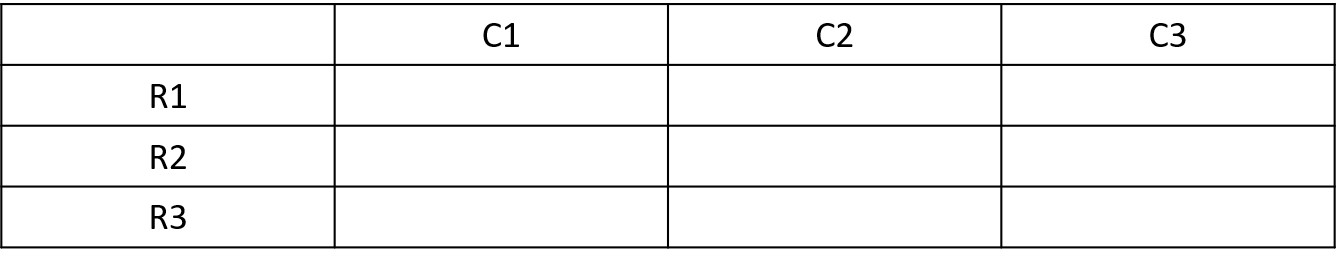
\includegraphics[scale = .5]{pic/question_2.png}
        \end{center}
        There should be at least one strategy being removed in each round. So, for player C,
        we need, at most 2 rounds to remove the other two strategies. So do player R.
        Then there should be at most 4 rounds in total to achieve the final decision.
        So, for a  \e{n \times n} game, with two players, there should be \e{n-1} rounds 
        for each player to drop all other strategies and remain only one strategy.
        Then, the upper bound for two-player iteration should be
        \ee{upper\_bound = (n - 1) + (n - 1) = 2 \times (n - 1)}.
        If there are k players in total, then the bound becomes
        \ee{upper\_bound = k \times (n - 1)}.

    \section{Question3}
        \subsection{(a) The order of elimination does not matter.}
            Clearly, for row player, $U > D$, for column player, $M > R$.\\

            1. If we remove D first:\\
            
            \begin{center}
                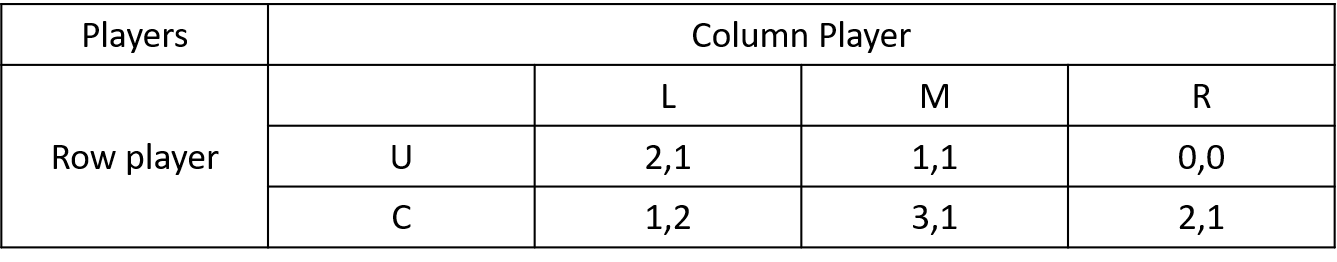
\includegraphics[scale = 0.5]{pic/remove_D_first.png}
            \end{center}
            
            And for column player, $L > M > R$.
            
            (1) If remove R first, 
            
            \begin{center}
                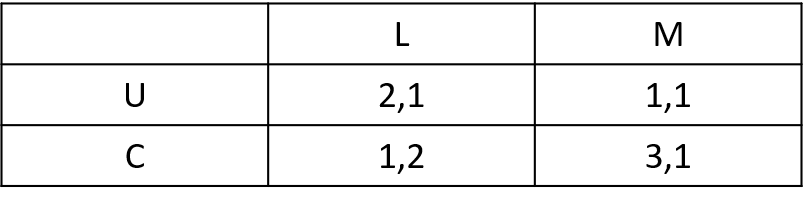
\includegraphics[scale = 0.5]{pic/remove_D_then_R.png}
            \end{center}
            
            Now, for column player, L is the dominant strategy. 
            Then, if L is chose, row player chooses U.
            The outcome is (U, L).\\

            (2) If remove M first,

            \begin{center}
                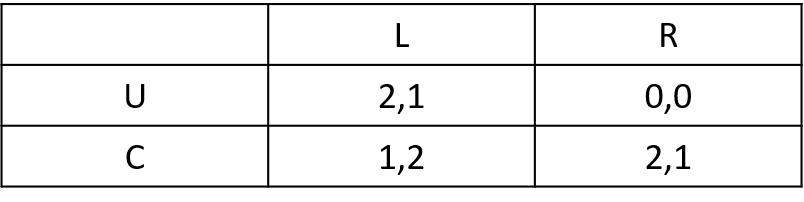
\includegraphics[scale = .5]{pic/remove_D_then_M.png}
            \end{center}
         
            L is still the dominant strategy.
            Then end up with (U, L).\\


            2. If remove R first:\\
            
            \begin{center}
                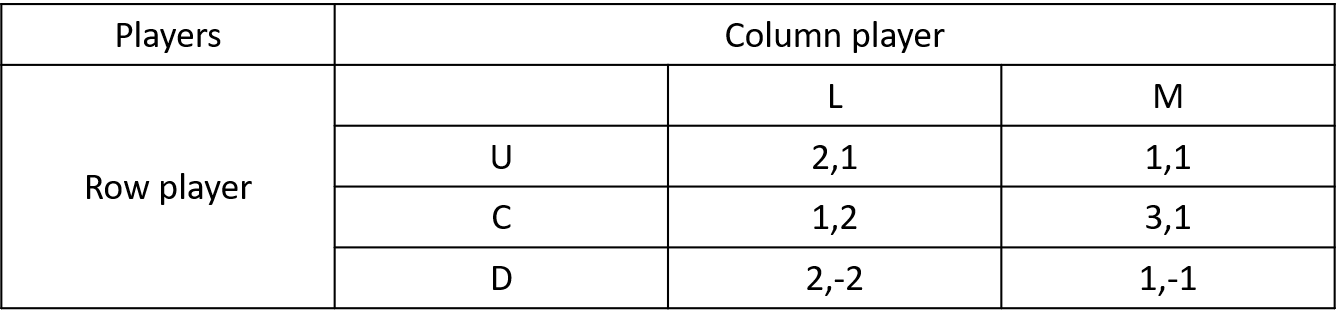
\includegraphics[scale = 0.5]{pic/remove_R_first.png}
            \end{center}

            There is NO strictly dominated strategy for both players.
            Then, we should look at the best responses (BRs).\\

            \begin{center}
                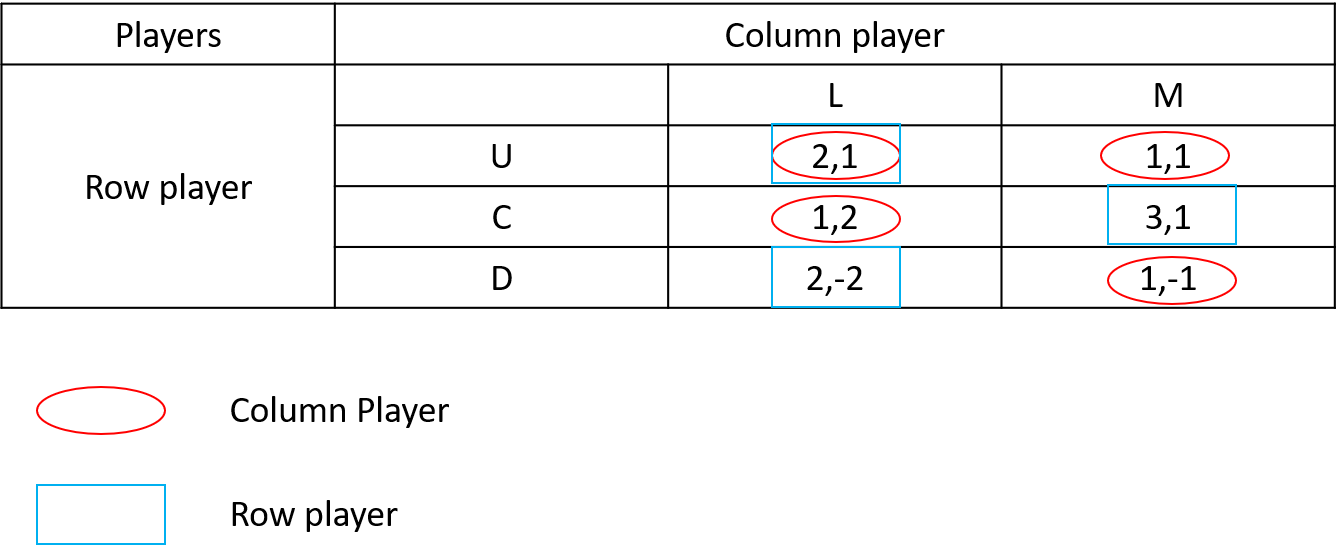
\includegraphics[scale = .5]{pic/outcome_reomve_R.png}
            \end{center}
            
            The game ends up with (U, L), because it is the mutual BR.\\
            But if we still using iteratively eliminating dominated strategy, for player R,
            the payoff for U and D are exactly the same no matter what C does.
            then, if we remove D, then, we end up with (U, L).
            However, if we remove U, we can make final decision.
            That's why order matters.
            \bb{Notice, weakly dominate only requires ''\e{\ge}'', it includes payoffs for 
            R along a row is exactly the same as payoffs in another row. So do player C (columns)}

            \begin{align*}
                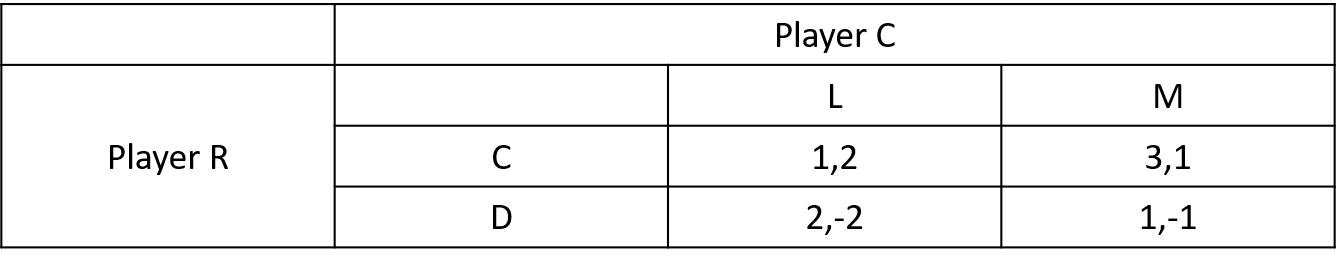
\includegraphics[scale = .5]{pic/unclear_remove.png}
            \end{align*}



        \subsection{(b) Proof}
            In static and complete information games, players know everything
            in the game. So, they should know what are the strictly dominated strategies
            for each player. Then, they do not need to consider the response to those strictly
            dominated strategies, because rivals will never choose those ones.
            Use this game as an example, the game actually starts with only U, C, L, M, a $2 \times 2$
            games rather $3 \times 3$

            \begin{center}
                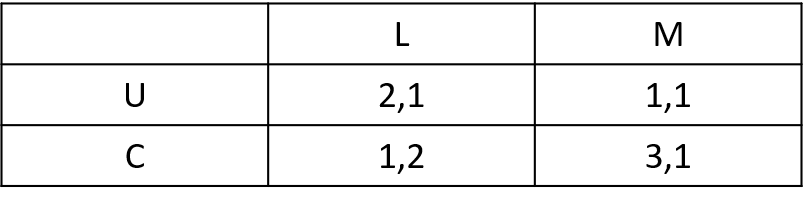
\includegraphics[scale = .5]{pic/2by2_game.png}
            \end{center}

            Then we can find, for column player, M is the strictly dominated strategy.
            So, he will only choose L. Then, row player chooses U as response.\\
    
    \section{Question4}

        Define $\hat{s}$ as a weakly \underline{undominated} strategy, and $\bar{s}$
        as some other strategies. We call $\hat{s}$ as weakly undominated if
        $$ u_i (\hat{s_i}, s_{-i}) \ge u_i(\bar{s_i}, s_{-i}).$$
        So,  $\hat{s_i}$ survives the iterative weak dominance. It means that there
        is at least one cell for this strategy is greater or equal to some other strategy $s_i$.
        Otherwise, $$u_i(\hat{s_i}, s_{-i}) < u_i(s_i, s_{-i}) \quad  \forall s_i\in S_i $$
        $\hat{s_i}$ is strictly dominated by $s_i$.
        Then, it is impossible for \e{\hat{s_i}} to be a strictly dominated strategy.
        %比如s_hat 是某一列,那么这一列中至少有一个单元格的值是比其所在行中其他单元格的值要大的。
        %不然他就是strictly dominated, 会在iterated中被淘汰。
        
\end{spacing}
\end{document}
